
Instead of setting up all possible Slater determinants, construct only an approximation to the ground state (where we assume that the four particles are in the two lowest single-particle orbits only) which includes at most two-particle-two-hole excitations.
Diagonalize this matrix and compare with the exact calculation and comment your results.
Can you set up which diagrams this approximation corresponds to?

\subsection{}
From Fig.~\ref{fig:SDs} we see that all states except $\ket{\Phi_5}$, has states with at most one pair of electrons above the $p=2$.
Our new approximation of the ground state is then shown in Fig.~\ref{fig:c_groundstate}.

\begin{figure}[htbp]
    \centering
    \includegraphics{figures/c_ground_state_energy.pdf}
    \caption{
        Ground state energy of the Hamiltonian matrix for the four-particle system with no broken pairs and total spin $S = 0$, as a function of the pairing strength $g$.
        Truncated to only include at most two-particle-two-hole excitations.\label{fig:c_groundstate}
    }
\end{figure}

As the figure shows, the approximate energies are very close, regardless of whether we include the four-particle state $\ket{\Phi_5}$ or not.

\begin{figure}[htbp]
    \centering
    \includegraphics{figures/c_diff_ground_state_energy.pdf}
    \caption{
        Difference in ground state energy of the Hamiltonian with all states below $p=4$ and the Hamiltonian with $\ket{\Phi_5}$ removed, as a function of the pairing strength $g$.
        Truncated to only include at most two-particle-two-hole excitations.\label{fig:c_diff_groundstate}
    }
\end{figure}

% TODO: Comment on differences

% \textcolor{red}{TODO:\@ MAKE DIAGRAMS}

\begin{figure}
    \centering
    \usetikzlibrary{decorations.markings}

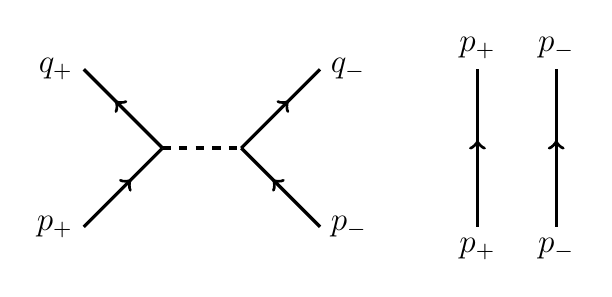
\begin{tikzpicture}[
        cross/.style={
            cross out,
            draw=black,
            minimum size=2*(#1-\pgflinewidth),
            inner sep=0pt,
            outer sep=0pt
        }, %default radius will be 1pt.
        cross/.default={1pt}
    ]

    \begin{scope}[very thick,decoration={
                markings,
                mark=at position 0.6 with {\arrow{>}}
            }
        ]
        \coordinate (upleft) at (0, 2) {};
        \coordinate (downleft) at (0, 0) {};
        \coordinate (midleft) at (1, 1) {};
        \coordinate (midright) at (2, 1) {};
        \coordinate (upright) at (3, 2) {};
        \coordinate (downright) at (3, 0) {};

        \draw[postaction={decorate}]   (downleft) node[left] {\large$p_+$} -- (midleft);
        \draw[postaction={decorate}]   (midleft) -- (upleft) node[left] {\large$q_+$};
        \draw[dashed] (midleft) -- (midright);
        \draw[postaction={decorate}]   (downright) node[right] {\large$p_-$} -- (midright) ;
        \draw[postaction={decorate}]   (midright) -- (upright) node[right] {\large$q_-$};

    \end{scope}

    \begin{scope}[xshift=5cm,very thick,decoration={
                markings,
                mark=at position 0.55 with {\arrow{>}}
            }
        ]
        \coordinate (upleft) at (0, 2) {};
        \coordinate (downleft) at (0, 0) {};
        \coordinate (upright) at (1, 2) {};
        \coordinate (downright) at (1, 0) {};

        \draw[postaction={decorate}]   (downleft) node[below] {\large$p_+$} -- (upleft) node[above] {\large$p_+$};
        \draw[postaction={decorate}]   (downright) node[below] {\large$p_-$} -- (upright) node[above] {\large$p_-$};
    \end{scope}
\end{tikzpicture}

% \end{document}

    \caption{
        Diagrams corresponding to the approximation of the ground state with at most two-particle-two-hole excitations.\label{fig:2p2h}
    }
\end{figure}
